% Modelo de slides para projetos de disciplinas do Abel
\documentclass[10pt]{beamer}

\usetheme[progressbar=frametitle]{metropolis}
\usepackage{appendixnumberbeamer}
\usepackage[numbers,sort&compress]{natbib}
\bibliographystyle{plainnat}

\usepackage{booktabs}
\usepackage[scale=2]{ccicons}

\usepackage{xspace}
\newcommand{\themename}{\textbf{\textsc{metropolis}}\xspace}

\AtBeginSection[]
{
  \begin{frame}
    \frametitle{Table of Contents}
    \tableofcontents[currentsection]
  \end{frame}
}




\title{TURLA\\LIGHTNEURON}
\subtitle{One email away from remote code execution}
% \date{\today}
\date{}
\author{Mario Leonardo Salinas}
\institute{UniPi - ICT Risk Assessment}
% \titlegraphic{\hfill\includegraphics[height=1.5cm]{logo.pdf}}

\begin{document}

\maketitle

\begin{frame}{Table of contents}
  \setbeamertemplate{section in toc}[sections numbered]
  \tableofcontents[hideallsubsections]
\end{frame}
%============================
%   1. Introduction
%============================
\section{Introduction}

\begin{frame}[fragile]{Metropolis}
  The \themename theme is a Beamer theme \cite{greenwade93} with minimal visual noise
  inspired by the \href{https://github.com/hsrmbeamertheme/hsrmbeamertheme}{\textsc{hsrm} Beamer
  Theme} by Benjamin Weiss. \cite{Er01}

  Enable the theme \cite{Simpson} by loading

  \begin{verbatim}    \documentclass{beamer}
    \usetheme{metropolis}\end{verbatim}

  Note, that you have to have Mozilla's \emph{Fira Sans} font and XeTeX
  installed to enjoy this wonderful typography.
\end{frame}
%============================
%   2. Attacker Profile & Victimology
%============================
\section{Attacker Profile \& Victimology}

\begin{frame}[fragile]{Attacker Profile i}
  \begin{itemize}
    \item Turla is well known for its advanced custom tools and its ability to run highly targeted operations.
    \item The group is interested in collecting information from strategic people
    or organizations.
  \end{itemize}
  \begin{figure}
    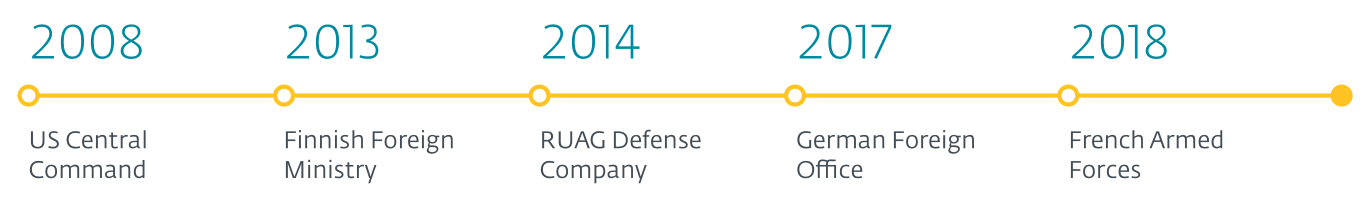
\includegraphics[width=\textwidth]{figures/timeline.PNG}
    \caption{Timeline of important attacks attributed to Turla}
  \end{figure}
\end{frame}

\begin{frame}[fragile]{Attacker Profile ii}
    \begin{itemize}
      \item The operators activity matches a typical 9-to-5 workday in the UTC+3 time zone
      \item LightNeuron is used mostly to exfiltrate data. The remaining activity is most likely dropping
      and executing tools to perform lateral movements across the local network
    \end{itemize}
    \begin{figure}
      \centering
      \subfloat[Operators working hours\label{fig:a}]{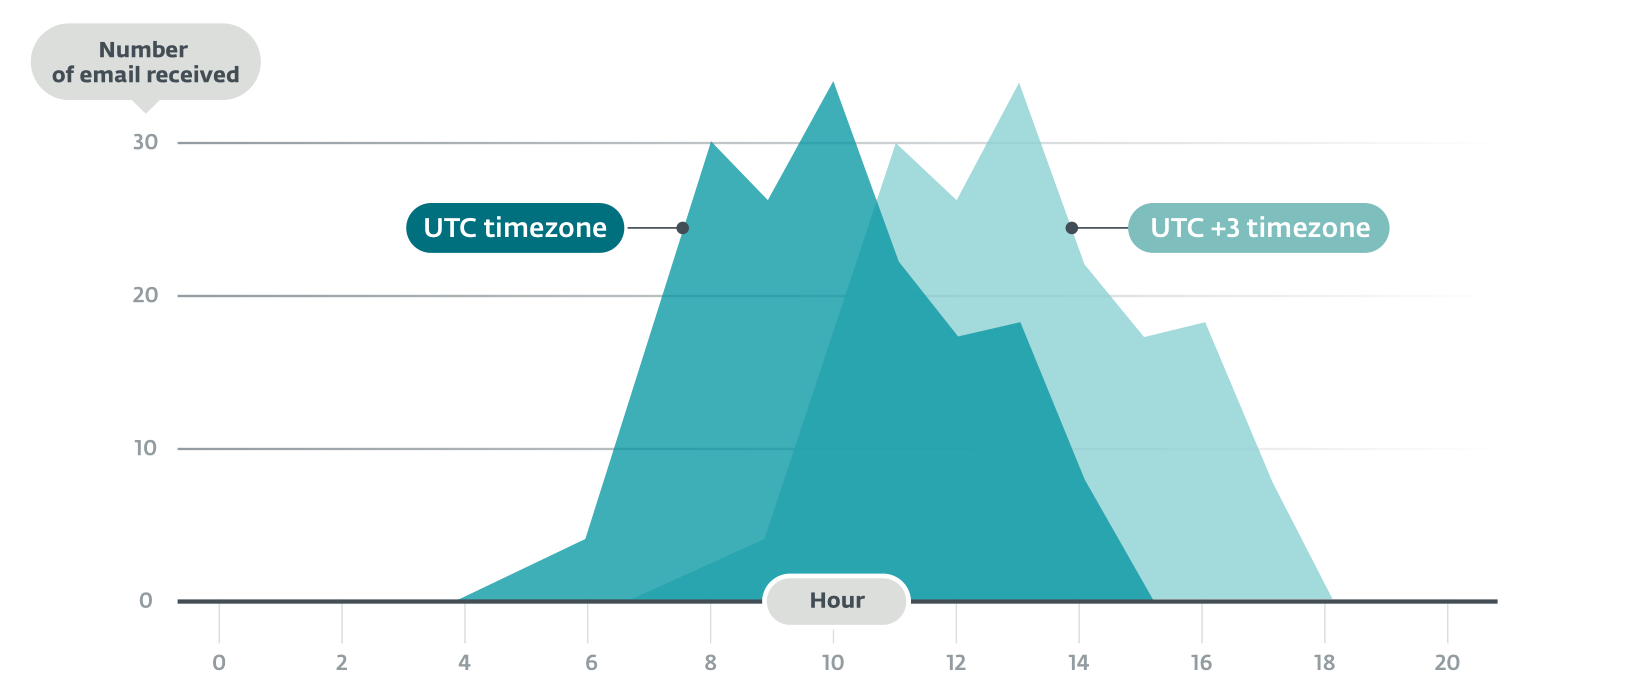
\includegraphics[height=3.5cm,width=5.5cm]{figures/attacker_timeline.PNG}}\qquad
      \subfloat[Distribution of the backdoor commands used by the operators\label{fig:b}]{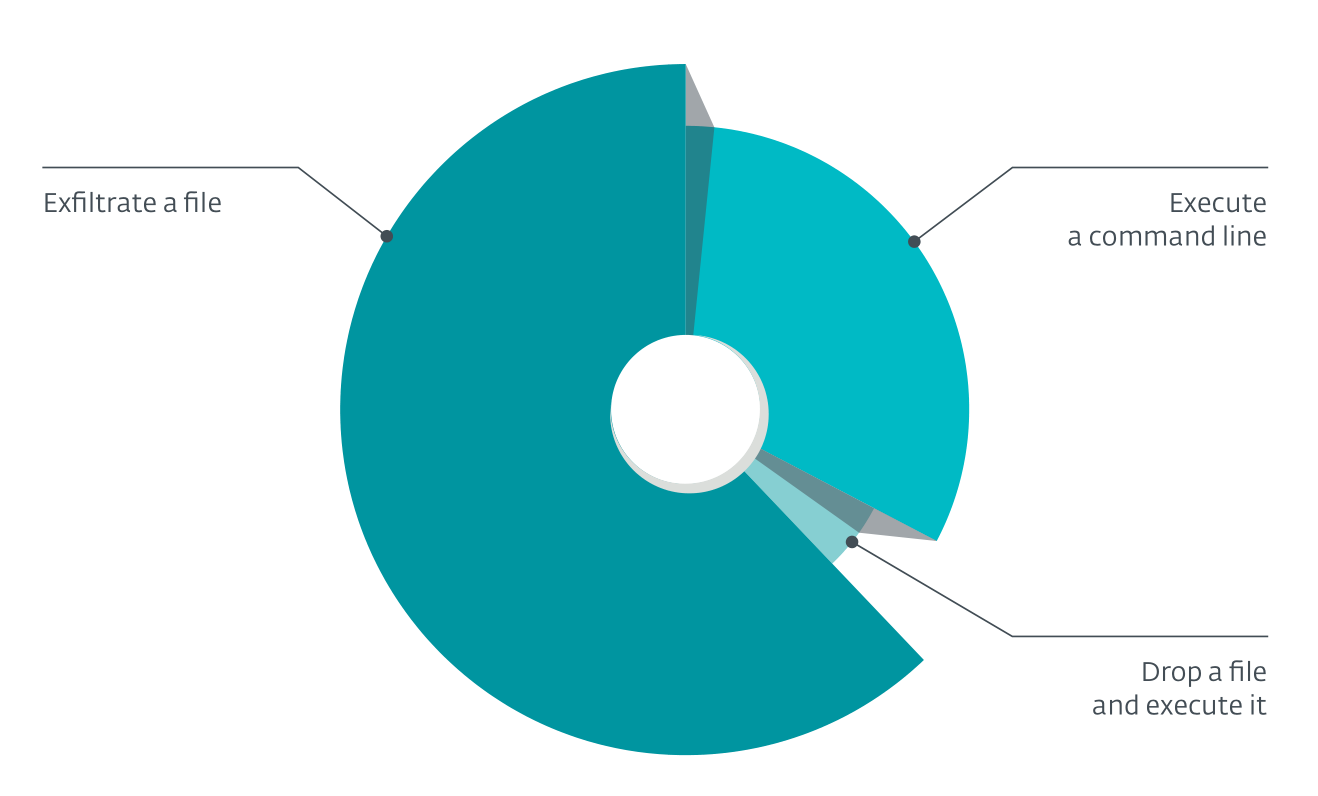
\includegraphics[height=3.5cm,width=4.6cm]{figures/commands_distrib.PNG}}
    \end{figure}
\end{frame}

\begin{frame}[fragile]{Victimology}
  According to ESET, LightNeuron development started before 2014; even if the development occurred
several years ago, LightNeuron is still used in recent compromises. These targets are in line with traditional Turla targets:
\begin{figure}
  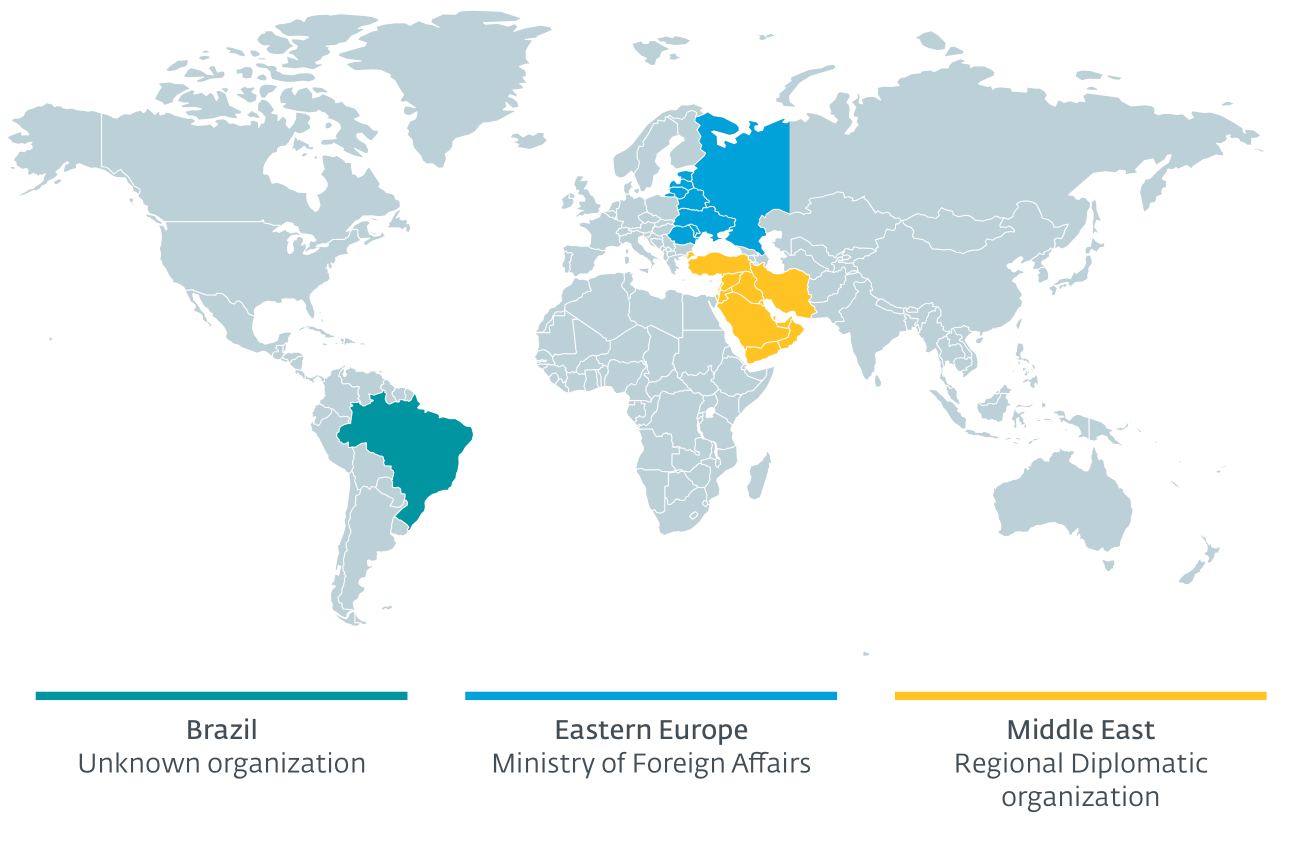
\includegraphics[width=8cm]{figures/map.PNG}
  \caption{Map of known LightNeuron victims}
\end{figure}
\end{frame}




%============================
%   Biblio
%============================

\begin{frame}[allowframebreaks]{References}

  \bibliography{demo}
  
  %\bibliographystyle{abbrv}

\end{frame}

\end{document}
